
%(BEGIN_QUESTION)
% Copyright 2012, Tony R. Kuphaldt, released under the Creative Commons Attribution License (v 1.0)
% This means you may do almost anything with this work of mine, so long as you give me proper credit

Mange brennbare gasser dannes som «avfallsprodukter» i kjemisk prosessindustri og oljeraffinerier. Disse «avfallsgassene» kan brukes som brensel for dampkjeler og forbrenningsovner i andre deler av raffineriet. Problemet er at produksjonen av «avfalls»-brenselgass ofte er ujevn, og etterspørselen etter brenselgass i kjeler og ovner er også ujevn. Noen ganger blir det overskudd av avfallsgass (mer enn det som kan brukes), og andre ganger blir det for lite.

Følgende trykkreguleringssystem arbeider for å holde et konstant brenselgasstrykk i akkumulatortanken til tross for endringer i avfallsgassflow og brenselgassbehov:

$$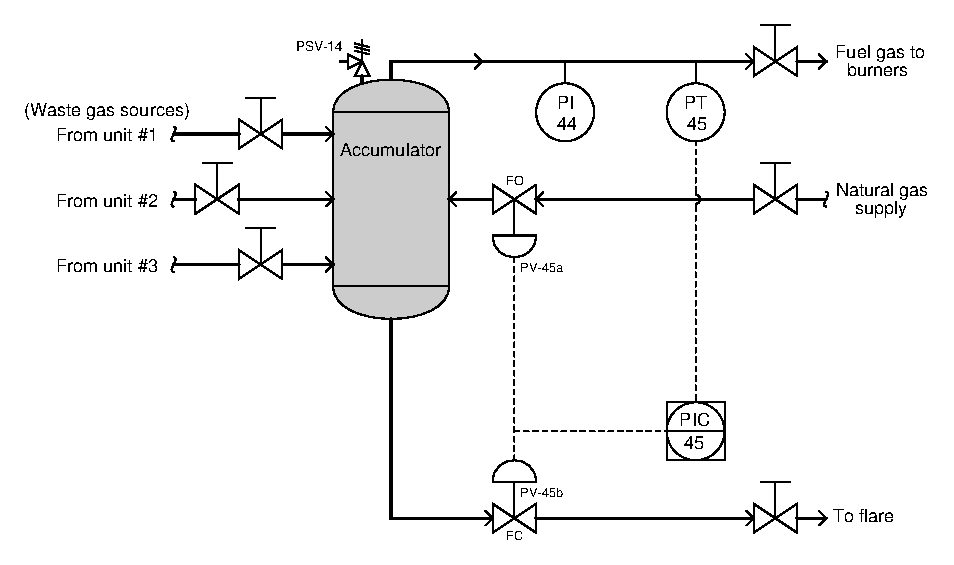
\includegraphics[width=15.5cm]{i01263x01.eps}$$

Et par split-range-reguleringsventiler (PV-45a og PV-45b) arbeider sammen for enten å slippe naturgass inn i akkumulatoren (når gasstrykket er for lavt) eller slippe overskuddsgass til fakkel (når trykket er for høyt).

\vskip 10pt

Driftspersonell har fastslått at trykket inne i denne akkumulatoren ikke er stabilt nok for deres driftsbehov. De har også fastslått at raske endringer i avfallsgassflow er kilden til ustabiliteten, og derfor ber de instrumentpersonell om å implementere en løsning. Instrumentpersonellet bestemmer seg for å implementere en {\it feedforward}-strategi for å møte dette behovet.

Første steg er selvsagt å installere flowmålere på hver av avfallsgasslinjene inn til akkumulatoren; signalene fra disse skal brukes i feedforward-strategien for å kompensere proaktivt for endringer i avfallsgassflow. Det oppstår imidlertid en uenighet mellom ansatte i instrumentavdelingen om hvordan feedforward-strategien skal implementeres.

\filbreak

Det ene teamet sier at strategien bør se slik ut:

$$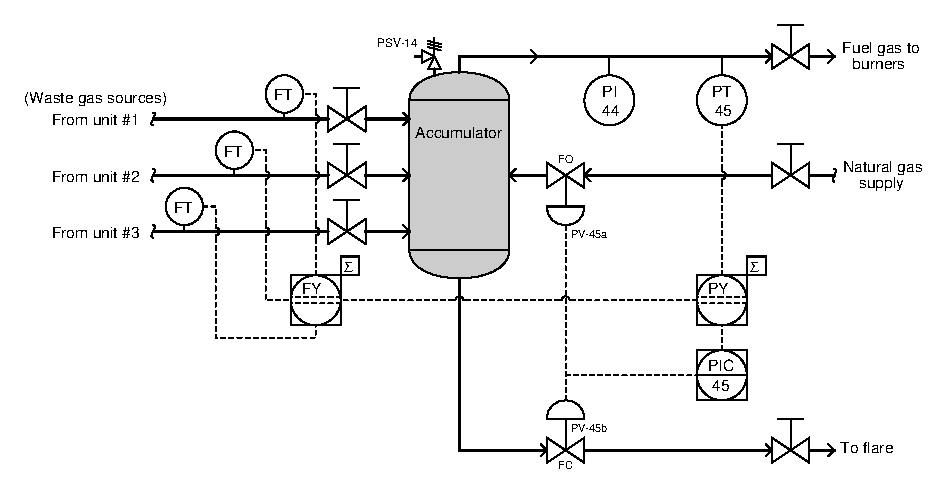
\includegraphics[width=15.5cm]{i01263x02.eps}$$

Det andre teamet sier at strategien bør se slik ut:

$$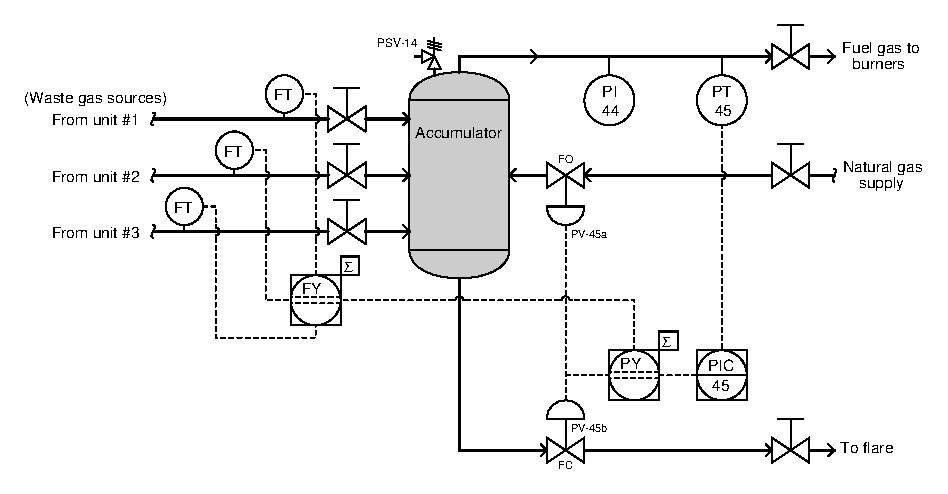
\includegraphics[width=15.5cm]{i01263x03.eps}$$

Hvilket team er du enig med, og hvorfor? Merk: {\it dette er et svært viktig konsept å forstå i feedforward-strategier, og faktisk et av de mest misforståtte konseptene knyttet til feedforward!}

\vskip 10pt

\underbar{file i01263}
%(END_QUESTION)





%(BEGIN_ANSWER)

Dette er den riktige løsningen, der signalet for total lastflow legges til {\it utgangen} fra trykkregulatoren, ikke til {\it PV-inngangen}:
 
$$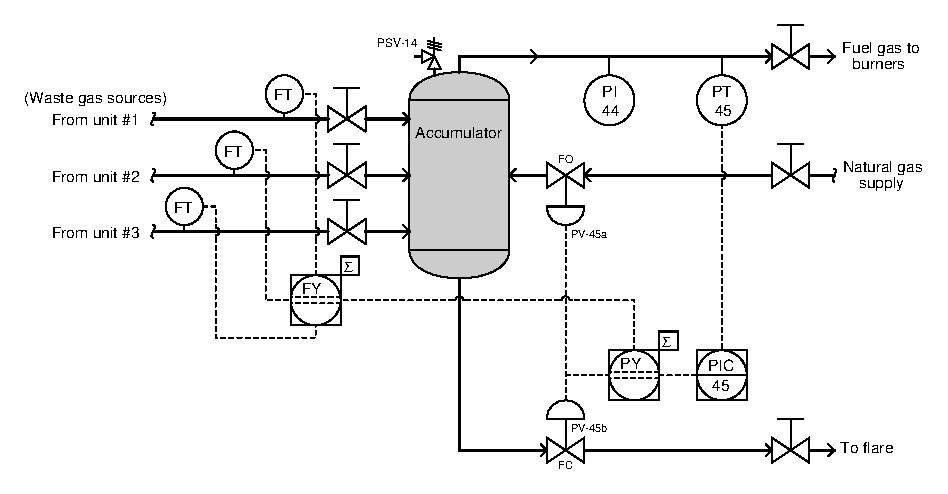
\includegraphics[width=15.5cm]{i01263x03.eps}$$

Årsaken er ganske enkel: vi ønsker at feedforward-signalet skal bidra direkte til reguleringsventilenes stilling, slik at enhver endring i avfallsgassflow umiddelbart påvirker ventilene for proaktiv kompensasjon. Hvis feedforward-signalet ble lagt til trykkregulatorens PV-signal, ville det få trykkregulatoren til å «se» trykkendringer som i virkeligheten er endringer i avfallsgassflow. Dette ville ikke bare unnlatt å gi ønsket effekt, men også «løyet» for trykkregulatoren, med det resultat at den aldri kunne holde setpunktet korrekt!

%(END_ANSWER)





%(BEGIN_NOTES)

$$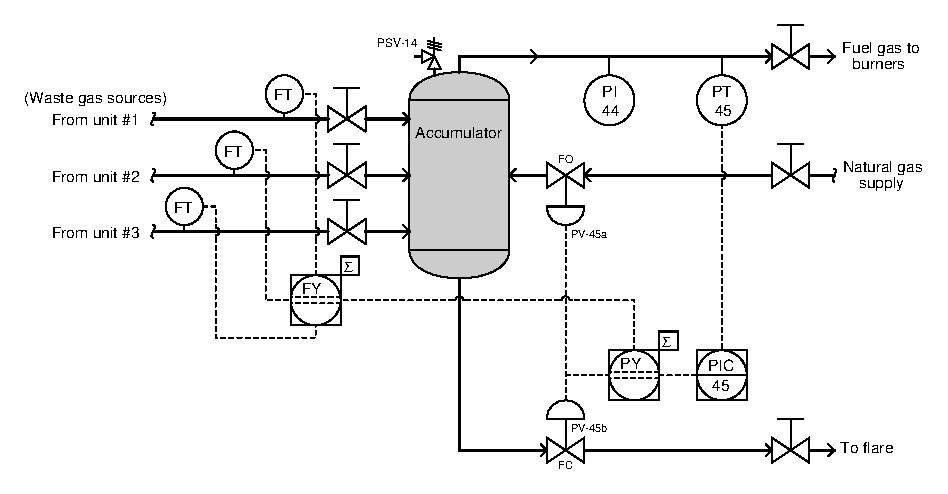
\includegraphics[width=15.5cm]{i01263x03.eps}$$

\vskip 20pt \vbox{\hrule \hbox{\strut \vrule{} {\bf Virtuell feilsøking} \vrule} \hrule}

\noindent
{\bf Forutsi virkningen av en gitt feil:} presenter hver av følgende feil for studentene, én om gangen, og la dem kommentere alle effektene hver feil vil gi.

\begin{itemize}
\item{} 
\item{} 
\item{} 
\end{itemize}


\vskip 10pt


\noindent
{\bf Identifisere mulige/umulige feil:} presenter symptomer for studentene og la dem deretter avgjøre om en serie foreslåtte feil kan forklare alle symptomene, og forklare {\it hvorfor} eller {\it hvorfor ikke} for hver foreslått feil:

\begin{itemize}
\item{} Symptom: {\it }
\item{}  -- {\bf Ja/Nei}
\item{}  -- {\bf Ja/Nei}
\item{}  -- {\bf Ja/Nei}
\end{itemize}


\vskip 10pt

\filbreak


\noindent
{\bf Vurdere nytten av gitte diagnostiske tester:} presenter symptomer for studentene og foreslå deretter følgende diagnostiske tester én etter én. Studentene vurderer verdien av hver test og avgjør om den vil gi nyttig informasjon (dvs. fortelle oss noe vi ikke allerede vet). Studentene avgjør hva ulike resultater for hver test i så fall kan indikere om feilen:

\begin{itemize}
\item{} Symptom: {\it PT-45 viser et oscillerende trykk}
\item{} Kontroller gain-verdier i FY-summer -- {\bf Nei}
\item{} Kontroller gain-verdi for PIC-45-summer -- {\bf Ja}
\item{} Sjekk PI-44-visning for å se om den også oscillerer -- {\bf Nei} (svært usannsynlig at PT-45 oscillerer av seg selv)
\item{} Undersøk faseskift mellom PV og utgang fra PIC-45 -- {\bf Ja}
\item{} Plott lastflow i en trendgraf -- {\bf Ja}
\end{itemize}


\vskip 10pt


\noindent
{\bf Diagnostisere en feil basert på gitte symptomer:} tenk deg at ??? feiler ??? i dette systemet (ikke avslør feilen til studentene!). Presenter operatørens observasjon(er) for studentene, la dem vurdere mulige feil og diagnostiske strategier, og fortell dem deretter resultatene av testene de foreslår basert på følgende symptomer, helt til de korrekt har identifisert feilens art og plassering:

\begin{itemize}
\item{} Operatørobservasjon: {\it }
\item{} 
\item{} 
\end{itemize}
%INDEX% Control, strategies: feedforward (gas accumulator pressure control)

%(END_NOTES)

